% -------------------------
% INTRODUCTION
% -------------------------

\graphicspath{{./\figurefolder/1Introduction/}}
% ----------------------------------------------------------------------------------------------------
% 0. Front Matter
% ----------------------------------------------------------------------------------------------------

\chapter{Introduction}\label{chap:0_intro}
\thispagestyle{empty}

% ----------------------------------------------------------------------------------------------------
% 1. Motivation
% ----------------------------------------------------------------------------------------------------
\newpage
\section{Background and Motivation} \label{sec:intro_motivation}
    Our world faces urgent societal challenges necessitating innovative solutions, including population growth, urbanization, low construction industry productivity, and escalating environmental impact in the building sector. The UN predicts the global population will reach 9.8 billion by 2050 \citep{united_nations_world_2019}, with global urbanization projected to increase from 56\% in 2020 to 68\% in 2050 \citep{ritchie_urbanization_2024}. This unprecedented urbanization trend becomes clear when viewed historically over the last several centuries, as depicted in \Cref{fig:intro_1}.
    
    \begin{figure}[ht]
    	\centering
    	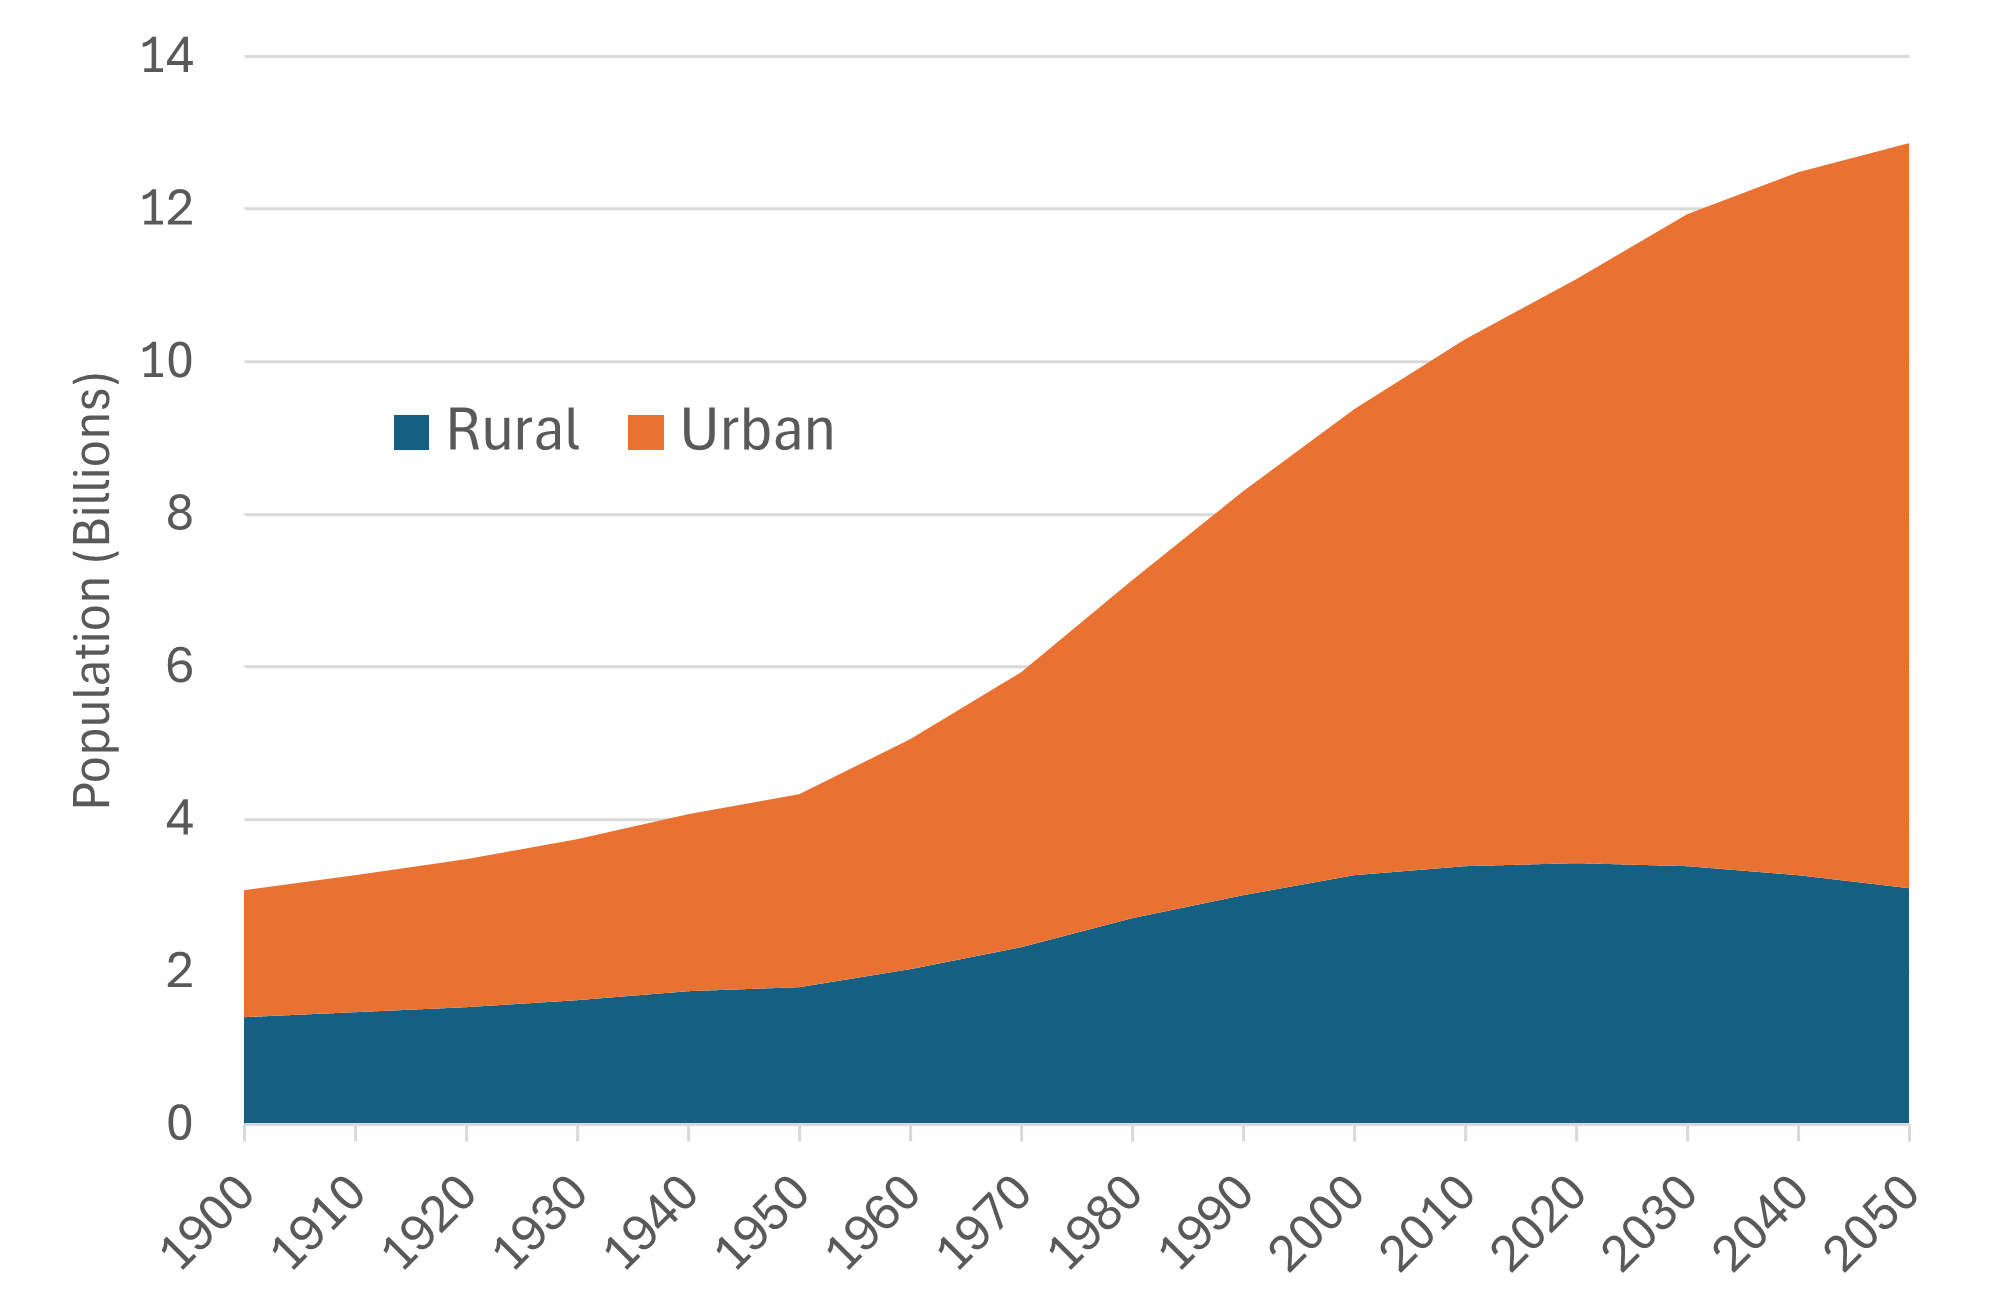
\includegraphics [trim={0cm 0.0cm 0cm 0.0cm}, clip, width=0.90\linewidth]{urban_rural_populations}
    	\caption{Total urban and rural populations given UN estimates from 1900-2023 and projections to 2050 base on UN median fertility scenario (data from \citep{ritchie_urbanization_2024})}
    	\label{fig:intro_1} 
    \end{figure}       
    
    Rapid population growth and urbanization are poised to drive increased demand for construction activities. However, the Architecture, Engineering, Construction (AEC) has a significant negative impact on the environment due to its material and energy-intensive manufacturing and construction processes \citep{international_energy_agency_2018_2018}, coupled with the high embodied carbon content of structural systems \citep{kaethner_embodied_2012, fang_reducing_2023}. For instance, buildings and construction activities contributed to 36\% of global energy usage and 37\% of global CO2 emissions in 2020, as depicted in \Cref{fig:intro_2} \citep{united_nations_global_2021}.

    \begin{figure}[ht]
    	\centering
    	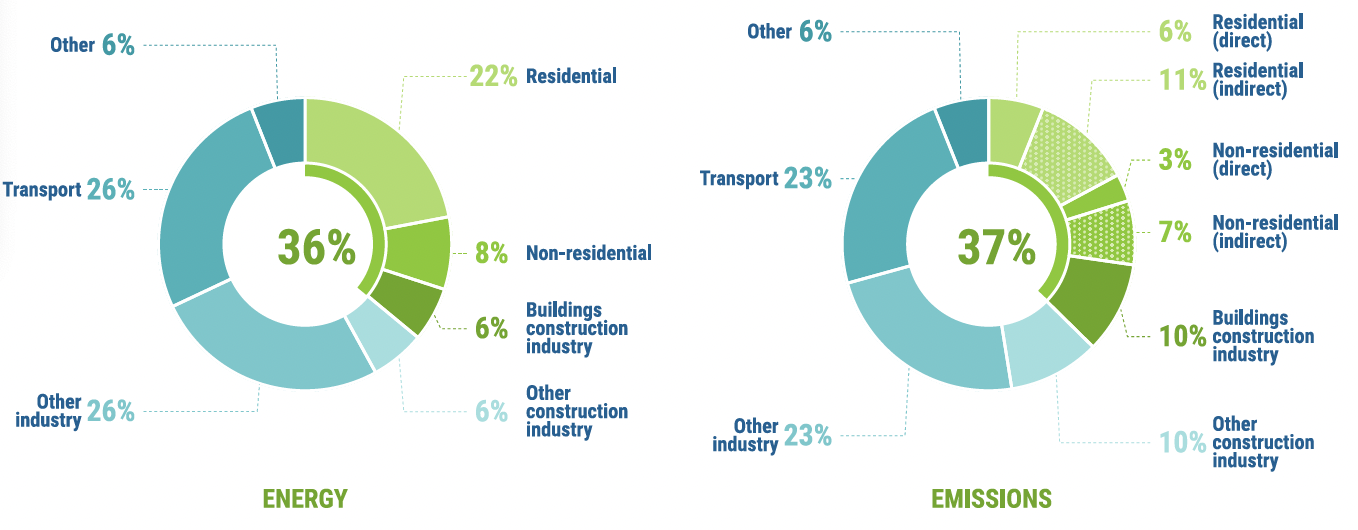
\includegraphics [trim={0cm 0.0cm 0cm 0.0cm}, clip, width=0.99\linewidth]{construction_percentages}
    	\caption{Construction industry's share of global energy use (left) and energy-related CO2 emissision (right) in 2020 (figure from \citep{united_nations_global_2021})}
    	\label{fig:intro_2} 
    \end{figure}   
    
    The environmental impact is further worsened by the increasing waste generated from construction and demolition (C\&D) processes \citep{us_epa_construction_2018, us_epa_construction_2020}. In the 1990s, C\&D processes were estimated to contribute up to 30\% of the total global waste \citep{purchase_circular_2022, fishbein_building_1998}. To illustrate this escalating issue, in the mid-1990s in the United States alone, C\&D activities generated an estimated 100-135 million tons of waste, of which about 35-45\% ended up in landfills \citep{mills_cost-effective_1999, us_epa_characterization_1998}. This C\&D waste accounted for 29\% of the total landfill volumes at that time \citep{lu_framework_2011}. However, by 2018, the volume of waste from C\&D activities had skyrocketed to 600 million tons, with 144 million tons or 24\% of this waste disposed of in landfills \citep{us_epa_advancing_2020}. Consequently, approximately half of the landfill volumes in 2018 were attributed to C\&D activities, while the remaining municipal solid waste contributed 146 million tons \citep{us_epa_advancing_2020}. This trend is especially concerning when considering the significant construction needs of the upcoming century, where aging infrastructure must be replaced while accommodating the demands of a growing and rapidly urbanizing global population \citep{ritchie_urbanization_2024}.

    As a result, inefficiencies within the AEC industry not only impede its ability to meet increasing demands but also exacerbate environmental degradation through wasteful practices and resource-intensive methods. Technological advancements aimed at enhancing construction efficiency and material utilization can mitigate some of these environmental impacts. However, the challenge lies in the AEC industry's reluctance to embrace contemporary automation techniques and the productivity benefits they offer. For instance, while various industries have witnessed an uptick in labor productivity since the 1940s, the construction sector has experienced only minor improvements and actually a decline in productivity since 1968, as illustrated in \Cref{fig:intro_3} \citep{barbosa_reinventing_2017}.

    \begin{figure}[ht]
    	\centering
    	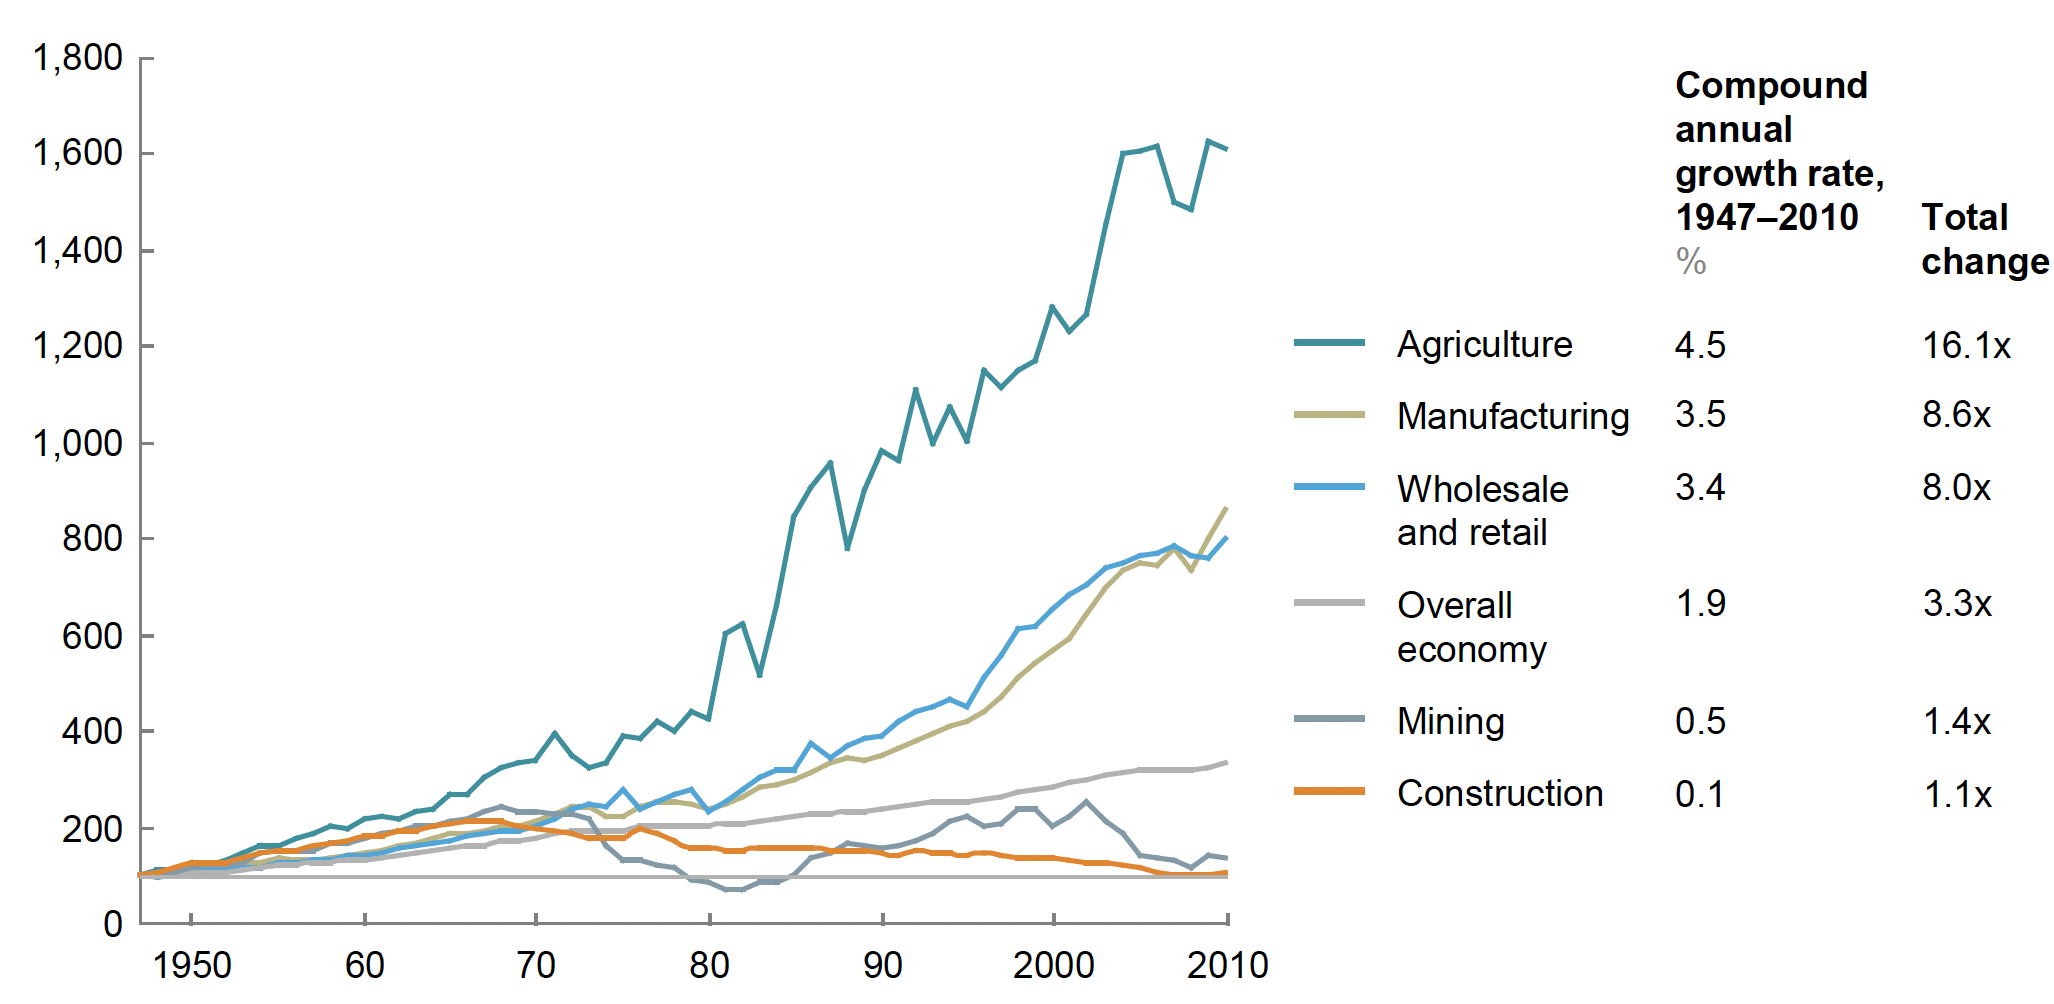
\includegraphics [trim={0cm 0.0cm 0cm 0.0cm}, clip, width=0.99\linewidth]{labor_productivity}
    	\caption{The productivity growth of several industries in the United States measured as gross value added per hour worked compared to a baseline of 100 measured in 1947 (figure from \citep{barbosa_reinventing_2017})}
    	\label{fig:intro_3} 
    \end{figure}  

\subsection{Broad Research Motivation stemming from Societal Challenges}
    The rapid increase in population growth and urbanization intensifies the need for construction activities, adding to the challenges already faced by the AEC industry, which struggles with stagnant productivity. This exacerbates environmental strain due to resource-intensive practices. While each challenge is significant on its own, their combined impact emphasizes the urgent requirement for changes in construction practices to promote sustainable development. It is crucial to adopt modern construction technologies that move away from wasteful and resource-intensive design approaches. Therefore, the broad motivation for the this dissertation is to:

    \begin{enumerate}
        \item Demonstrate the use of novel technologies that can be used by the construction industry to meet the growing demands of urbanization and population growth.
        \item Develop processes that enable the reduction of primary resource inputs to construction to minimize the environmental footprint of the building industry.
    \end{enumerate}

    % \begin{figure}[ht]
    % 	\centering
    % 	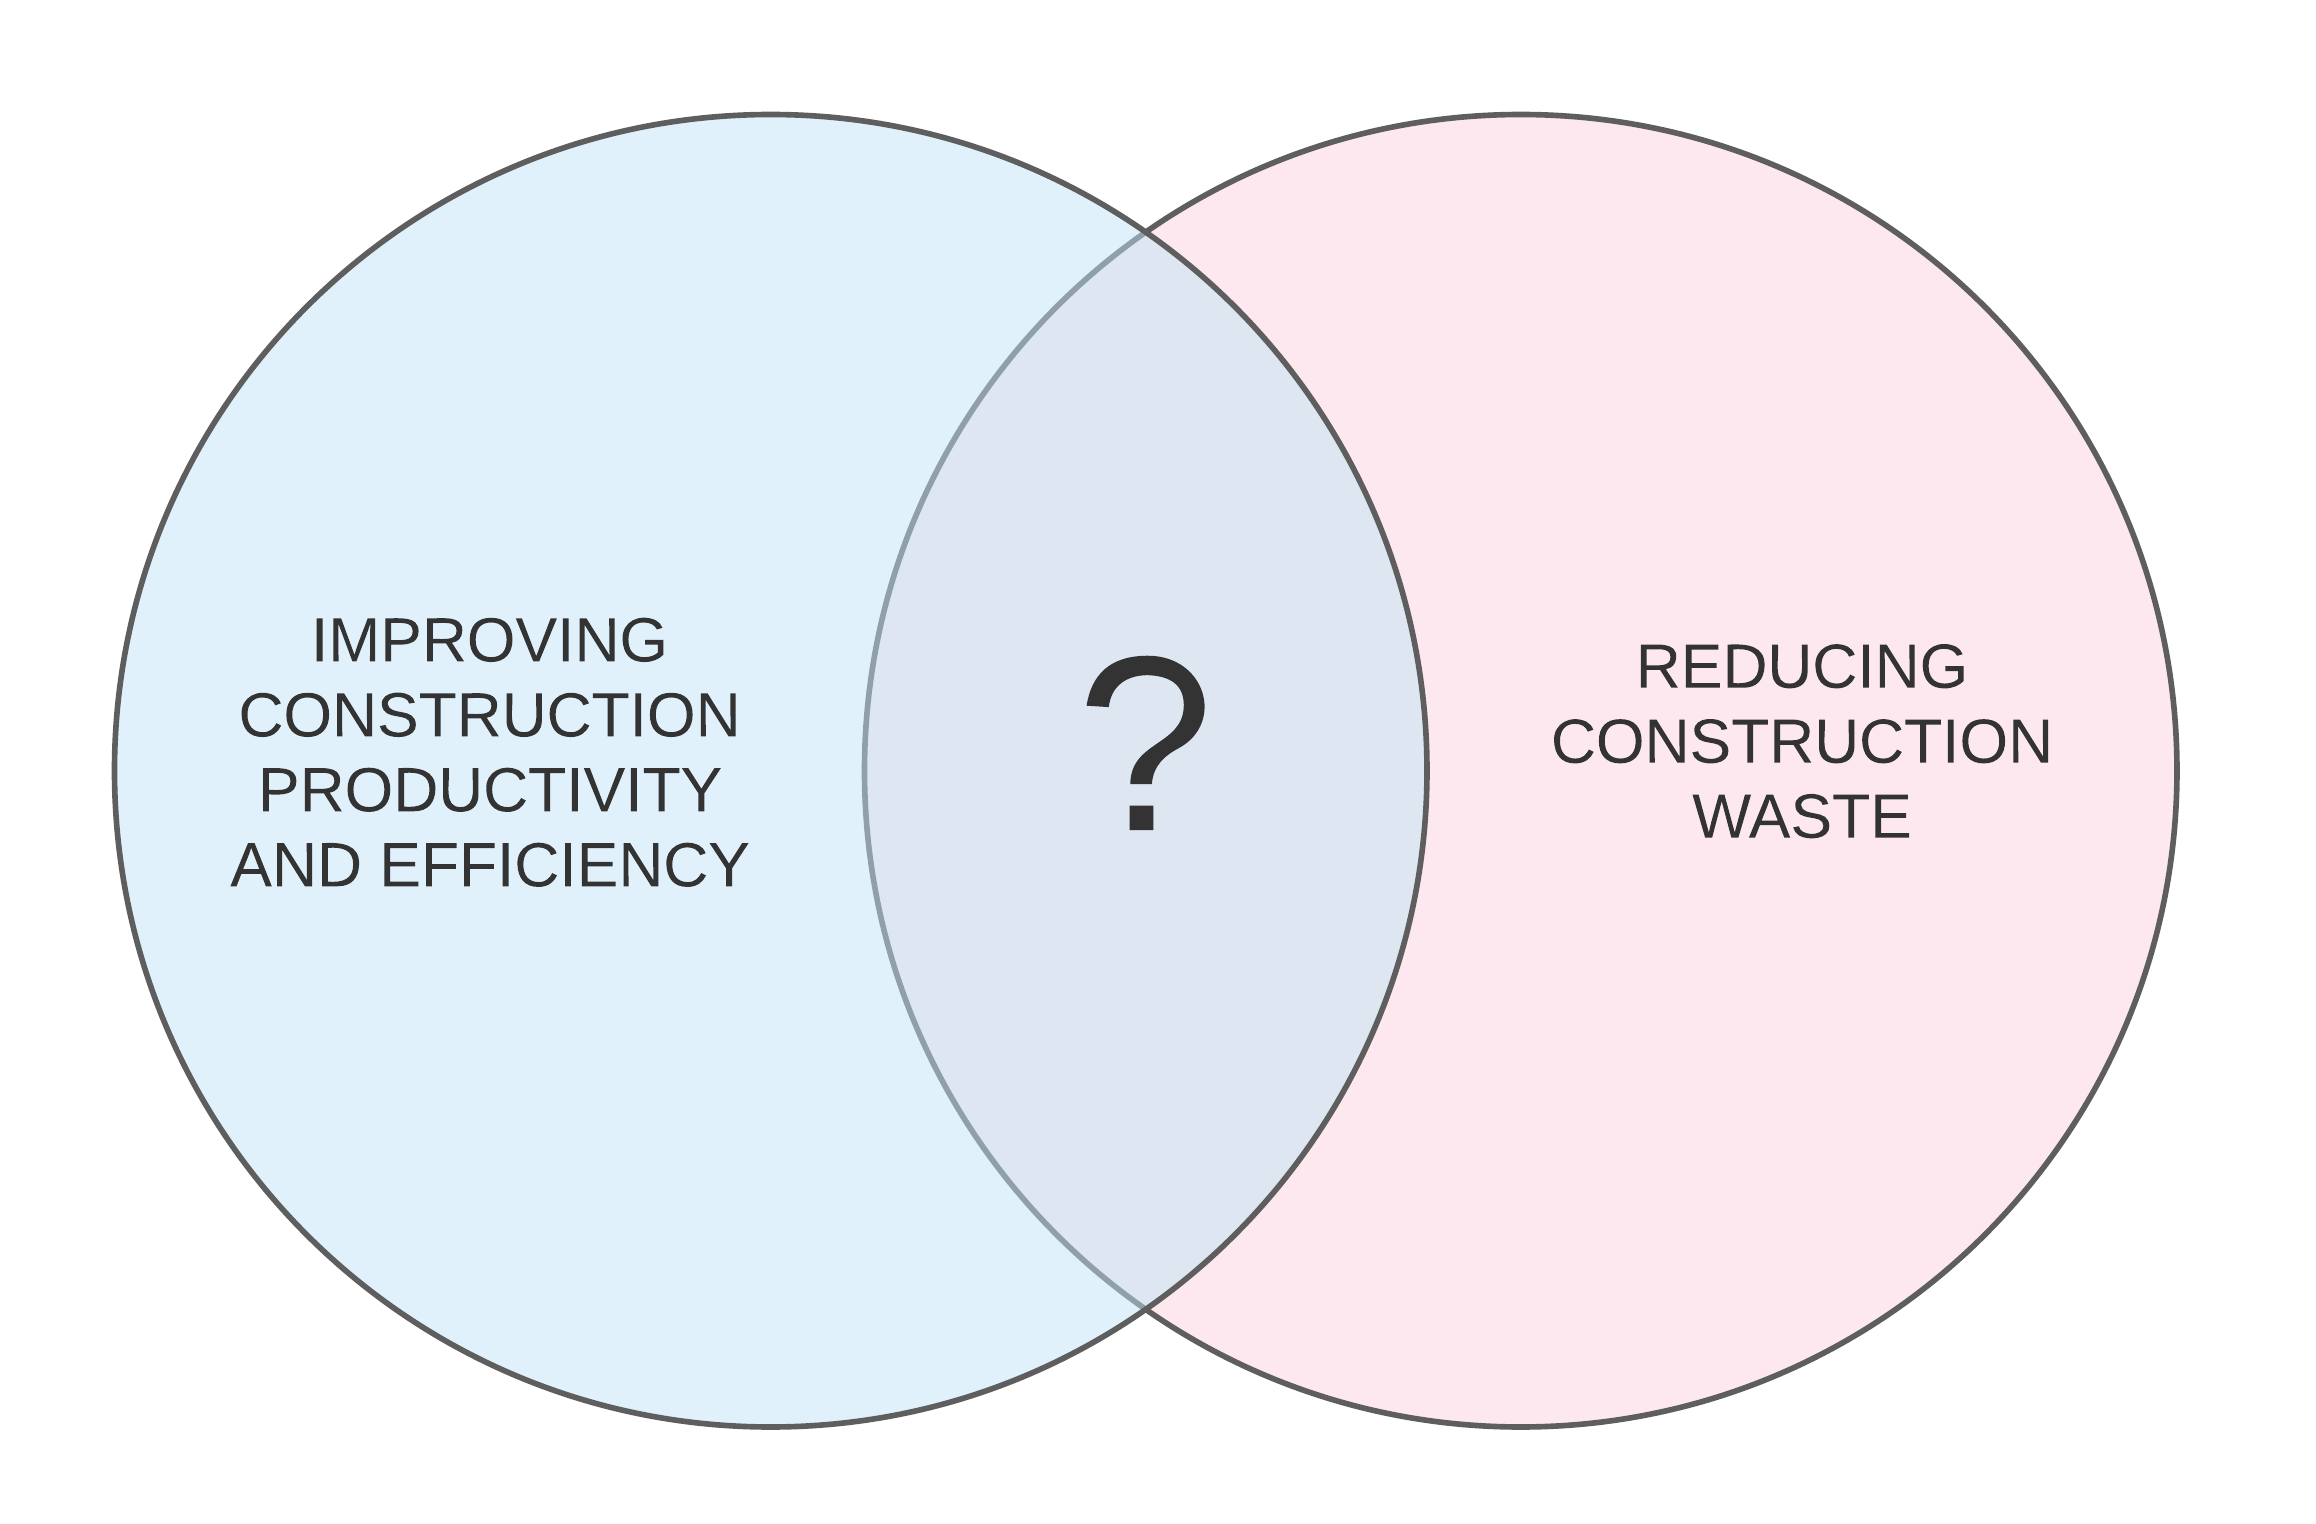
\includegraphics [trim={0cm 0.0cm 0cm 0.0cm}, clip, width=0.85\linewidth]{motivation}
    % 	\caption{Research objectives motivation stemming from AEC-specific societal challenges.}
    % 	\label{fig:intro_4} 
    % \end{figure}  


% ----------------------------------------------------------------------------------------------------
% 1. Research Objectives
% ----------------------------------------------------------------------------------------------------
\section{Research Objectives}
    The research goal of this dissertation, derived from the broad research motivations and the societal challenges outlined in \Cref{sec:intro_motivation}, is to demonstrate how robotic construction automation can be used to perform various construction tasks in such a way that makes external supports (such as scaffolding) unnecessary. Industrial robots are particularly applicable to construction of discrete element structures due to their application versatility \citep{bravo-palacios_one_2020} and spatial precision in picking and placing material \citep{eversmann_robotic_2017}. They are experiencing growing adoption in both industry and academic contexts \citep{ifr_world_2018} and have already shown promise in tackling the AEC industry's lagging productivity and labor efficiency \citep{garcia_de_soto_productivity_2018, kumar_robotics_2016}.

    This dissertation specifically explores the use of cooperative robotic fabrication (CRF) as a design approach and construction method. In CRF setups, individual robotic agents are sequenced to work together, improving productivity by allowing for the automation of a wider range of construction tasks, including intricate pick-and-place processes. Furthermore, the dissertation showcases how CRF can advance the adoption of sustainable circular models in building design and construction. This is achieved by minimizing primary resource consumption during construction and facilitating disassembly and reuse processes. A thorough literature review of CRF can be found in \Cref{chap:2_context}, which provides information about CRF in this specific research context.
    
    The dissertation focuses on the practical application of CRF as demonstrated in physical construction scenarios. The body of the dissertation is organized as a series of research chapters demonstrating increasingly intricate uses of CRF methodologies across various construction contexts, involving different materials, and structural typologies. Across all research, the central theme is utilizing CRF setups to execute construction tasks without the need for additional external temporary support materials, essentially maintaining stability without relying on formwork or scaffolding during any stage of construction. Multiple robots are strategically coordinated to collaborate in adding or removing structural elements while providing necessary support to the temporary structure independently. In each research project, this type of cooperative robotic sequencing is leveraged, where a team of two or more robots execute multiple tasks simultaneously, or perform complimentary passive/active functions, in coordinated manner to achieve scaffold-free behavior. The research presented in this dissertation starts with assembly-only applications, but increase in complexity to include applications of disassembly as well. By integrating disassembly into the design and fabrication process, opportunities for future structural reconfiguration and reuse within a circular economy framework are explored and demonstrated.
    
    The overall goal of demonstrating CRF's potential to improve construction productivity through automation while highlighting applications for it to be used for material reduction and circular models of construction, is achieved through the following specific research objectives:
    
    \begin{enumerate}
        \item Develop a structurally-informed support-place sequencing method for cooperative robotic construction processes that allows for the scaffold-free (de)construction of spanning (i.e., arches, vaults, frames etc.) as opposed to vertical or layer-based structures.
        \item Demonstrate CRF in increasingly complex applications for different structural typologies and material systems:
            \begin{enumerate}
                \item small-scale test of human-robot collaborative assembly
                \item assembly of masonry vaults and arches
                \item (dis)assembly of space frames designed for reversibility
                \item dis-and-reassembly of existing timber stick frames
            \end{enumerate}
        \item Establish future research directions and applications of the developed CRF method
    \end{enumerate}



% ----------------------------------------------------------------------------------------------------
% Significance of Research
% ----------------------------------------------------------------------------------------------------  
\section{Novelty and Significance of Research}
    While the use of robots and construction automation gained prominence initially in the 1970s with single-task robots used for the prefabrication of modular homes in Japan \citep{bock_construction_2007, bock_future_2015, bock_construction_2016, albus_trip_1986}, it was only in the last two decades that the Digital Fabrication (DFab) movement in construction began to gain significant attention \citep{gramazio_digital_2008}. As part of this movement researchers have aimed to expand the geometric design possibilities and productivity in construction through the utilization of robots for bespoke structures \citep{gramazio_made_2014, davila_delgado_robotics_2019}.
    
    Despite the strides made in the DFab movement, robotic fabrication's application to discrete element structures remains predominantly focused on vertical layer-based construction \citep{bartschi_wiggled_2010, kohler_gantenbein_2014, bonwetsch_informed_2006, bonwetsch_digitally_2007, piskorec_brick_2018, dorfler_mobile_2016, giftthaler_mobile_2017}. This dissertation represents a significant departure from this convention by presenting the first examples of assembling various types of spanning structures, rather than vertical or layer-based ones, at the architectural pavilion scale, without the need for external scaffolding or support. Additionally, this research broadens the scope of CRF methods by successfully applying them to scaffold-free disassembly and reassembly for the first time. These advancements build on the first demonstrated examples of scaffold-free cooperative robotic assembly, for vertical steel spatial structures, in the PhD work of Parascho \citep{parascho_cooperative_2019}.

    In addition, this dissertation explores CRF for the first time through the lens of resource-informed design. Resource-informed design integrates considerations of assembly and disassembly processes directly into the design of structures, as illustrated in a simple design loop in \Cref{fig:intro_4}. Addressing waste begins at the design phase, where strategic planning can significantly reduce material usage and waste generation throughout the project life cycle. Research indicates that a notable portion of construction waste stems from inadequate waste reduction measures early in the design stages, particularly in planning for building decommissioning \citep{osmani_architects_2008}. Resource-informed design involves developing connections between the structure and fabrication setups to maximize cooperative potential, thereby optimizing efficiency and reducing resource inputs during fabrication. This approach aims to minimize the use of structural materials, temporary scaffolding, and manual labor while facilitating the reuse of materials, thus promoting sustainability and moving away from single-use construction practices. Overall, resource-informed design seeks to create structures that are not only functional and aesthetically pleasing but also efficient, sustainable, and adaptable throughout their life cycle.

    \begin{figure}[ht]
    	\centering
    	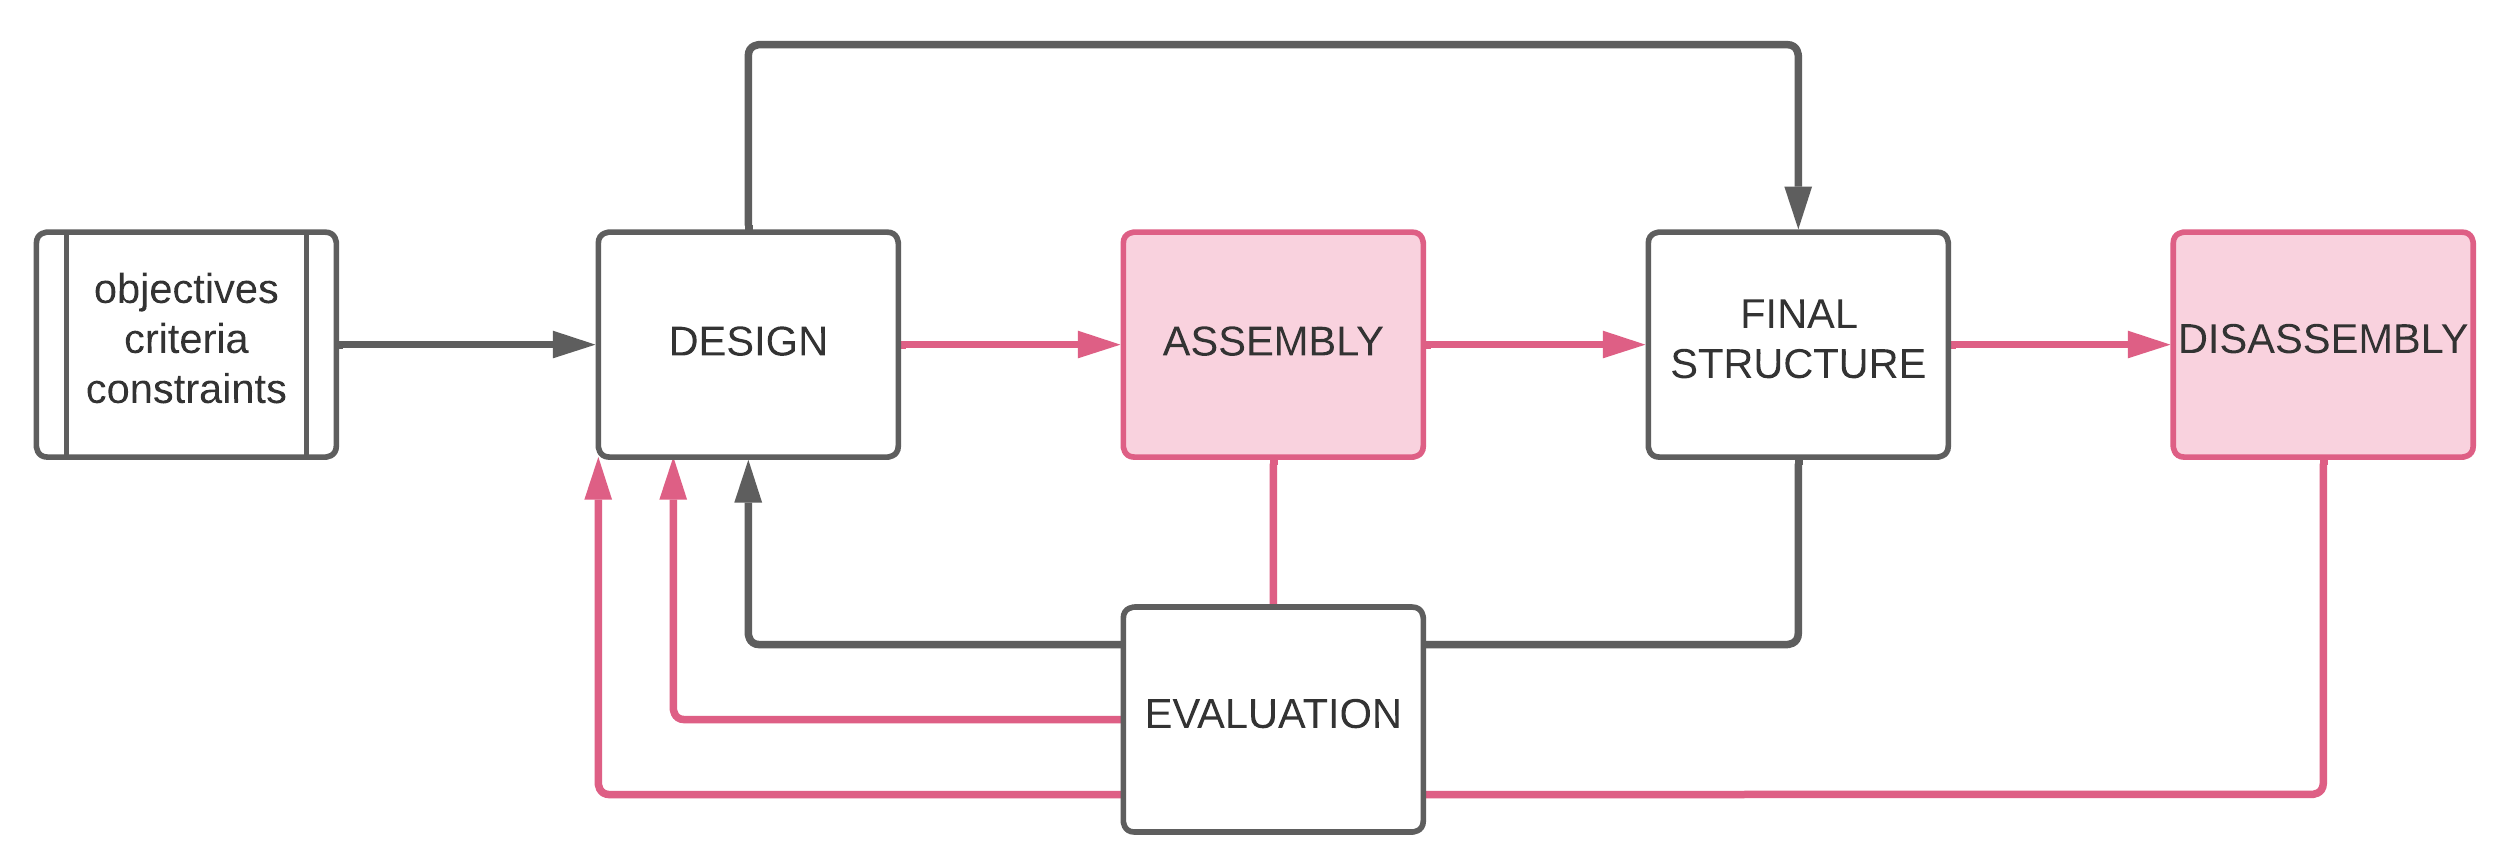
\includegraphics [trim={0cm 0.0cm 0cm 0.0cm}, clip, width=0.99\linewidth]{fab_informed}
    	\caption{Resource-informed design framework including implicit considerations for assembly and disassembly.}
    	\label{fig:intro_4} 
    \end{figure}  
    

% ----------------------------------------------------------------------------------------------------
% Dissertaton Structure and Organization
% ----------------------------------------------------------------------------------------------------  
% \newpage
\section{Dissertation Structure and Organization}
    Through a series of independent research projects, this dissertation develops and demonstrates the application of CRF for scaffold-free construction. Given the diversity of structural and material types, and construction scopes explored, a project-specific literature review is provided at the beginning of each chapter. The organization of this dissertation is as follows:
    
    \Cref{chap:2_context} functions as a general literature review and introduces CRF as a technology and reviews its previous applications across industries, with a focus on applications in the built environment. It explores the idea that CRF has the potential to achieve outcomes that align with certain aspects in the transition towards circular economic practices, as demonstrated in the research presented in the upcoming chapters.
    
    \Cref{chap:3_humanrobot} introduces a novel bottom-up design framework where robots actively participate in the creative design process, detailing the cooperative aggregation of solid spherical units by two robotic arms to create a branching spatial structure assembled without requiring external scaffolding.
    
    \Cref{chap:4_LightVault} explores the use of multiple robots in cooperative assembly to construct complex spanning masonry structures without scaffolding, presenting and validating three fabrication approaches and demonstrating an optimized method for scaffold-free construction of a stable masonry arch.
    
    \Cref{chap:5_SpaceFrame} presents a fabrication-informed design method for stable  triangulated space frame structures, utilizing a graph theoretic framework to specifically design a rigidity-preserving spanning structure that can be assembled and disassembled without external scaffolding using two cooperating robots.
    
    \Cref{chap:6_ZeroWaste} showcases how CRF enables the disassembly and reuse of existing timber buildings, demonstrating the development and use of the support hierarchy graph for planning different disassembly and reassembly sequences using up to 3 robots working together.
    
    \Cref{chap:7_conclusion} summarizes the body of the dissertation consisting of the four independent research projects and their contributions to advancing the various circular economy principles as outlined in Chapter 2, while discussing future directions for scaffold-free assembly and disassembly research utilizing CRF methods.



% ----------------------------------------------------------------------------------------------------
% Prior Work
% ----------------------------------------------------------------------------------------------------  
% \newpage
\section{Prior Publications Contributing to this Dissertation}
    Except for this introductory chapter, all subsequent chapters in this dissertation comprise previously published peer-reviewed materials such as book chapters, journal papers, or conference papers. To maintain clarity of authorship, only publications where the author of this dissertation serves as the first and corresponding author are incorporated. These relevant publications are referenced at the outset of each chapter and are included with the publishers' consent. Additionally, the contributions of co-authors of these publications are recognized through a CRediT (Contributor Roles Taxonomy) author statement at the commencement of each chapter \citep{allen_how_2019}. Minor adjustments from the original publication may have been made to align the content with the overall formatting requirements of this dissertation and to ensure stylistic coherence across chapters.
    
    For a comprehensive compilation of all peer-reviewed publications pertaining to the dissertation's themes, authored or co-authored by the dissertation's author during the course of this degree, please refer below. This list encompasses co-authored works that, although not directy integrated into the body of this dissertation, bear significant relevance to its thematic focus and feature substantial contributions from the author.
    
    \vspace{0.5cm}
    \noindent\textbf{Book Chapters}
    \begin{enumerate} [topsep=0pt]
        \item \textbf{Bruun, E. P. G.}, Parascho, S., \& Adriaenssens, S. (2024). Cooperative Robotic Fabrication for a Circular Economy. In A Circular Built Environment in the Digital Age (pp. 129–149). Springer Cham. https://doi.org/10.1007/978-3-031-39675-5\_8
    \end{enumerate}

    \vspace{0.5cm}
    \noindent\textbf{Peer-Reviewed Journal Papers}
    \begin{enumerate} [topsep=0pt]
        \item \textbf{Bruun, E. P. G.}, Adriaenssens, S., Besler, E., \& Parascho, S. (2024). ZeroWaste: Disassembly and Reuse of a Timber Frame Structure using Cooperating Robots. Construction Robotics. (Accepted)
        %
        \item \textbf{Bruun, E. P. G.}, Oval, R., Al Asali, W., Gaspar, O., Paris, V., \& Adriaenssens, S. (2024). Automating historical centering-minimizing masonry vaulting strategies: Applications to cooperative robotic construction. Developments in the Built Environment. (Under Review)

        \item Oval, R., Paris, V., Pastrana, R., \textbf{Bruun, E. P. G.}, Gomis Aviño, S., Adriaenssens, S., \& Al Asali, W. (2024). Digital guidework for augmented thin-tile vaulting construction. Automation in Construction. (Under Review)

        \item Oval, R., Pastrana, R., \textbf{Bruun, E. P. G.}, Paris, V., Gomis Aviño, S., Adriaenssens, S., \& Al Asali, W. (2024). An integrated digital design and construction approach for falsework-minimal masonry vaults. Structures, 63, 106428. https://doi.org/10.1016/j.istruc.2024.106428
        %
        \item \textbf{Bruun, E. P. G.}, Adriaenssens, S., \& Parascho, S. (2022). Structural rigidity theory applied to the scaffold-free (dis)assembly of space frames using cooperative robotics. Automation in Construction, 141, 104405. https://doi.org/10.1016/j.autcon.2022.104405
        %
        \item \textbf{Bruun, E. P. G.}, Pastrana, R., Paris, V., Beghini, A., Pizzigoni, A., Parascho, S., \& Adriaenssens, S. (2021). Three cooperative robotic fabrication methods for the scaffold-free construction of a masonry arch. Automation in Construction, 129, 103803. \\ https://doi.org/10.1016/j.autcon.2021.103803
        %
        \item \textbf{Bruun, E. P. G.}, Ting, I., Adriaenssens, S., \& Parascho, S. (2020). Human–robot collaboration: A fabrication framework for the sequential design and construction of unplanned spatial structures. Digital Creativity, 31(4), 320–336. https://doi.org/10.1080/14626268.2020.1845214
        %
        \item Parascho, S., Han, I. X., Walker, S., Beghini, A., \textbf{Bruun, E. P. G.}, \& Adriaenssens, S. (2020). Robotic vault: A cooperative robotic assembly method for brick vault construction. Construction Robotics, 4(3), 117–126. https://doi.org/10.1007/s41693-020-00041-w
    \end{enumerate}
    
    \vspace{0.5cm}
    \noindent\textbf{Peer-Reviewed Conference Papers}
    \begin{enumerate} [topsep=0pt]

        % \item Al Asali, W., Oval, R., Pastrana, R., \textbf{Bruun, E. P. G.}, Paris, V., Gomis Aviño, S., \& Adriaenssens, S. (2024). Designing and Building in Dialogue: Augmented Reality for Masonry Vault Construction. Design Modelling Symposium: Scalable Disruptors. Design Modelling Symposium, Kassel. (Accepted)

        \item \textbf{Bruun, E. P. G.}, Adriaenssens, S., Besler, E., \& Parascho, S. (2022). ZeroWaste: Towards Computing Cooperative Robotic Sequences for the Disassembly and Reuse of Timber Frame Structures. Proceedings of the 42nd Annual Conference of the Association for Computer Aided Design in Architecture, 586–597. http://arks.princeton.edu/ark:/88435/pr1wp9t657
        %
        \item Paris, V., Lepore, N., \textbf{Bruun, E. P. G.}, Ruscica, G., Piccioni, M. D., Beghini, A., Parascho, S., \& Adriaenssens, S. (2021). Robotic construction of a self-balancing glass masonry vault: DEM study of stability during construction stages. Proceedings of the IASS Annual Symposium 2020/2021, 314–325. http://arks.princeton.edu/ark:/88435/pr12n4zh86
        %
        \item Parascho, S., Han, I. X., Beghini, A., Miki, M., Walker, S., \textbf{Bruun, E. P. G.}, \& Adriaenssens, S. (2021). LightVault: A design and robotic fabrication method for complex masonry structures. Advances in Architectural Geometry 2020, 350–375. \\ https://oar.princeton.edu/handle/88435/pr1s17ss
        %
        \item Han, I. X., \textbf{Bruun, E. P. G.}, Marsh, S., Adriaenssens, S., \& Parascho, S. (2020). From concept to construction: A transferable design and robotic fabrication method for a building-scale vault. Proceedings of the 40th Annual Conference of the Association for Computer Aided Design in Architecture, 614–623. \\ https://doi.org/10.52842/conf.acadia.2020.1.614
    \end{enumerate}


% ----------------------------------------------------------------------------------------------------
% Bibliography
% ----------------------------------------------------------------------------------------------------  
\newpage
\bibliographystyle{\BiblioPath/elsarticle-num} 

\begingroup
    \hypersetup{hidelinks} %turns off colors for URL and DOIs
    \bibliography{\BiblioPath/1Introduction}
\endgroup